%% LyX 2.4.4 created this file.  For more info, see https://www.lyx.org/.
%% Do not edit unless you really know what you are doing.
\documentclass[english,handout]{beamer}
\usepackage{mathptmx}
\usepackage[T1]{fontenc}
\usepackage[latin9]{inputenc}
\usepackage{amssymb}
\usepackage{cancel}
\PassOptionsToPackage{normalem}{ulem}
\usepackage{ulem}

\makeatletter
%%%%%%%%%%%%%%%%%%%%%%%%%%%%%% Textclass specific LaTeX commands.
% this default might be overridden by plain title style
\newcommand\makebeamertitle{\frame{\maketitle}}%
% (ERT) argument for the TOC
\AtBeginDocument{%
  \let\origtableofcontents=\tableofcontents
  \def\tableofcontents{\@ifnextchar[{\origtableofcontents}{\gobbletableofcontents}}
  \def\gobbletableofcontents#1{\origtableofcontents}
}

%%%%%%%%%%%%%%%%%%%%%%%%%%%%%% User specified LaTeX commands.
\usetheme{Warsaw}
% or ...

\setbeamercovered{transparent}
% or whatever (possibly just delete it)
\setbeamercovered{invisible} %makes overlays invisible

%gets rid of navigation symbols
\setbeamertemplate{navigation symbols}{}

%\usepackage{hyperref}
%\usepackage[usenames,dvipsnames,table]{xcolor} %adds additional color options
\definecolor{links}{HTML}{2A1B81}
%\hypersetup{colorlinks,linkcolor=blue,urlcolor=links}

\usepackage{multicol}

\usepackage{tikz}
\usetikzlibrary{calc}
\usetikzlibrary{plotmarks}
\usepackage{pgfplots}
\pgfplotsset{compat=newest}

\usepackage{calc}
\usepackage[nomessages]{fp}

%\usepackage{advdate}    % Advancing/saving dates
\usepackage{datetime}   % Dates formatting
%\usepackage{datenumber} % Counters for dates

\usepackage[super]{nth}

\usepackage{etex}

\usepackage[outline]{contour}  %allows text halos
\contourlength{1pt} %sets halo width
%%example: \node at (0.75,0.5) {\contour{white}{\Large Text!}};
%%example:  \node [fill=white,inner sep=1pt] at (2.25,0.5) {\Large 			Text!};
%%example:  \node [fill=white,rounded corners=2pt,inner sep=1pt] at 			(3.75,0.5) {\Large Text!};

%%%%%%%%%%%%%%%%%%%%%%%%%%%
\def\formatdateny{\csname noyear\languagename\expandafter\endcsname\formatdate}
\def\noyearenglish#1, \the\@year{#1}
\let\noyearamerican\noyearenglish
\let\noyearbritish\noyearenglish

%%%redefines column alignment to match vertically
%\define@key{beamerframe}{t}[true]{% top
  %\beamer@frametopskip=.2cm plus .5\paperheight\relax%
  %\beamer@framebottomskip=0pt plus 1fill\relax%
 % \beamer@frametopskipautobreak=\beamer@frametopskip\relax%
  %\beamer@framebottomskipautobreak=\beamer@framebottomskip\relax%
  %\def\beamer@initfirstlineunskip{}%
%}

%%provides pdf with 4 slides per page; don't forget to add 'handout' to remove overlays
\usepackage{pgfpages}
\pgfpagesuselayout{4 on 1}[a4paper, landscape, border shrink=7mm]
\pgfpageslogicalpageoptions{1}{border code=\pgfusepath{stroke}}
\pgfpageslogicalpageoptions{2}{border code=\pgfusepath{stroke}}
\pgfpageslogicalpageoptions{3}{border code=\pgfusepath{stroke}}
\pgfpageslogicalpageoptions{4}{border code=\pgfusepath{stroke}}
%%Don't forget to add 'handout'

\makeatother

\usepackage{babel}
\begin{document}
\newcommand{\xmax}{2000}
\newcommand{\xmin}{0}
\newcommand{\xstep}{0} %must be xmin+n
\newcommand{\ymax}{500}
\newcommand{\ymin}{0}
\newcommand{\ystep}{0} %must be ymin+n

\newcounter{countEx} \setcounter{countEx}{0}
\newcounter{countProb} \setcounter{countProb}{0}
\resetcounteronoverlays{countEx} \resetcounteronoverlays{countProb}

\newcommand{\ex}[3]{
	\addtocounter{countEx}{1}
	\only<#1-#2>{\begin{exampleblock} {Example \chNum.\secNum.\arabic{countEx}.} #3	\end{exampleblock}}
}

\newcommand{\prob}[4]{
	\addtocounter{countProb}{1}
	\only<#1-#2>{\begin{exampleblock} {Problem  \chNum.\secNum.\arabic{countProb}.\,#3} #4	\end{exampleblock}}
}

\newcommand{\yline}[4]{
	(#2 - #4)/(#1 - #3)*(x - #1) + #2
}

\beamerdefaultoverlayspecification{<+->}

%%%%Chapter and Section numbers%%%%%
\newcommand{\chNum}{2}
\newcommand{\secNum}{2}
\newcommand{\secTitle}{Applications of Venn Diagrams}

\title[Section \chNum.\secNum: \secTitle]{Section \chNum.\secNum: \secTitle}

\subtitle{Finite Mathematics~~MTH 107~~Fall 2014}

\author{Dr.\,James Ashe}

\titlegraphic{\includegraphics[height=2.75cm]{/home/jim/JamesAshe/MHU/images/MarsHilUniversityLogo-Virtical.png}}

\date{\formatdate{25}{8}{2014}}

\institute{Mars Hill University}

\makebeamertitle 
\begin{frame}{Review}

\begin{columns}


\column{6cm}
\begin{itemize}
\item <1->\emph{$A'$, complement} of $A$:

\begin{itemize}
\item <1->everything \uline{not}\emph{ }in $A$
\end{itemize}
\item []
\item <4->$X\subset A$\emph{, proper subset }of $A$:

\begin{itemize}
\item <5->Any subset of $A$ \uline{not equal to} \uline{\mbox{$A$}}\emph{.} 
\end{itemize}
\item []
\item <7->\emph{Improper subset }of $A$.

\begin{itemize}
\item <8->$A$ is the only one.
\end{itemize}
\item <10->$X\subseteq A$\emph{, subset }of $A$:

\begin{itemize}
\item <11->Any set that is contained in $A$.
\end{itemize}
\end{itemize}

\column{6cm}

\vspace{-10pt}
\begin{itemize}
\item <2->[ex.]Let $A=\{a,b,c\}$ and $U=\{a,b,c,d,e\}$
\item <3->[]$A'=\{c,d,e\}$
\item []
\item []
\item <6->[]$\emptyset,\{a\},\{b\},\{a,b\}\subseteq A$
\item []
\item []
\item <9->[]$\{a,b,c\}\subseteq A$ but $\{a,b,c\}\not\subset A$

\begin{itemize}
\item []
\item []\vfill
\end{itemize}
\end{itemize}
\end{columns}
\end{frame}

\begin{frame}{Counting: Two Sets}

\vspace{-.5cm}
\begin{columns}


\column{5.5cm}

\ex{1}{}{Of 100 houses, 76 have a DVD player, 21 have a Blue Ray player, and 12 have both.}
\begin{itemize}
\item <1->What is $U$?
\item <2->How many do not have a DVD player?

\begin{itemize}
\item <5->[]$n(U)-n(D)=n(D')$
\item []
\end{itemize}
\item <6->How many have a DVD or Blue Ray player?

\begin{itemize}
\item <9->[]$n(D\cup B)=n(D)+n(B)-n(D\cap B)$
\item []
\end{itemize}
\end{itemize}

\column{6cm}

%%%blank%%%
\only<1-2>{%%%%A uncolored; B uncolored%%%%%
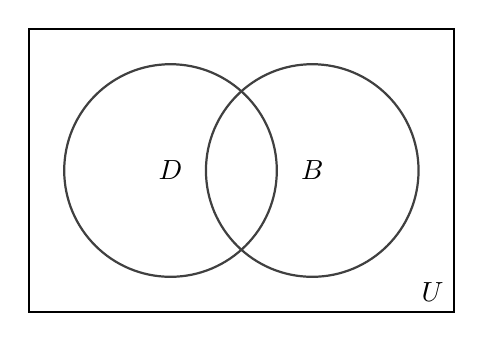
\begin{tikzpicture}[scale=.9]
	\def\circleA{(0,0) circle (1.5)} %A
	\def\circleB{(0:2) circle (1.5)} %B

	\colorlet{circle edgeA}{black!75} 
	\colorlet{circle areaA}{red!100}
	\colorlet{circle edgeB}{black!75} 
	\colorlet{circle areaB}{green!100}

	\tikzset{
		filledA/.style={fill=circle areaA, draw=circle edgeA, thick},
		filledB/.style={fill=circle areaB, draw=circle edgeB, thick},
		outlineA/.style={draw=circle edgeA, thick},
		outlineB/.style={draw=circle edgeB, thick},
	}

	\begin{scope}[fill opacity=0.5]         
			%\fill[filledB] \circleB;    
			%\fill[filledA] \circleA;
	\end{scope}

	\draw[outlineA] \circleA node {$D$}; 
	\draw[outlineB] \circleB node {$B$}; 
	%\node[anchor=south] at (current bounding box.north) {$A \cup B$}; 
	\draw[thick] (-2,-2) rectangle (4,2) node[anchor=south east] at (current bounding box.south east) {$U$}; 
\end{tikzpicture} }\only<3-5>{%%%%A complement%%%%%
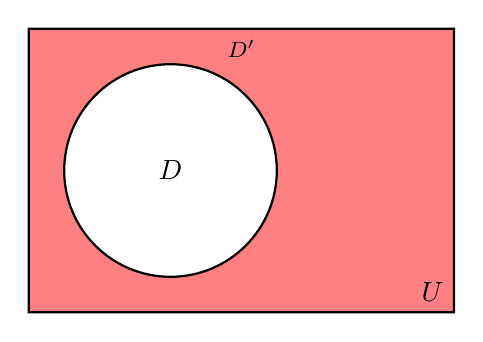
\begin{tikzpicture}[scale=.9]
	\def\circleA{(0,0) circle (1.5)} %A
	\def\circleB{(0:2) circle (1.5)} %B

	\colorlet{circle edgeA}{black!75} 
	\colorlet{circle areaA}{red!100}
	\colorlet{circle edgeB}{black!75} 
	\colorlet{circle areaB}{blue!100}

	\tikzset{
		filledA/.style={fill=circle areaA, draw=circle edgeA, thick},
		filledB/.style={fill=circle areaB, draw=circle edgeB, thick},
		outlineA/.style={draw=circle edgeA, thick},
		outlineB/.style={draw=circle edgeB, thick},
	}

	\draw[thick,fill=red!50,even odd rule] %%even odd rule draws complement of next draw commands%%
		(-2,-2) rectangle (4,2) node[anchor=south east] at (current bounding box.south east) {$U$} 
		\circleA node {$D$};
	\node[below=1pt] at (current bounding box.north) {\footnotesize $D'$}; 

\end{tikzpicture} }%%%blank%%%
\only<6-6>{%%%%A uncolored; B uncolored%%%%%
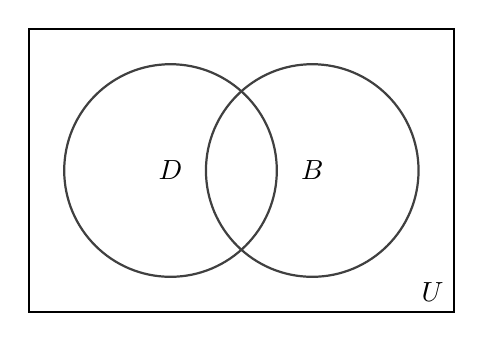
\begin{tikzpicture}[scale=.9]
	\def\circleA{(0,0) circle (1.5)} %A
	\def\circleB{(0:2) circle (1.5)} %B

	\colorlet{circle edgeA}{black!75} 
	\colorlet{circle areaA}{red!100}
	\colorlet{circle edgeB}{black!75} 
	\colorlet{circle areaB}{green!100}

	\tikzset{
		filledA/.style={fill=circle areaA, draw=circle edgeA, thick},
		filledB/.style={fill=circle areaB, draw=circle edgeB, thick},
		outlineA/.style={draw=circle edgeA, thick},
		outlineB/.style={draw=circle edgeB, thick},
	}

	\begin{scope}[fill opacity=0.5]         
			%\fill[filledB] \circleB;    
			%\fill[filledA] \circleA;
	\end{scope}

	\draw[outlineA] \circleA node {$D$}; 
	\draw[outlineB] \circleB node {$B$}; 
	%\node[anchor=south] at (current bounding box.north) {$A \cup B$}; 
	\draw[thick] (-2,-2) rectangle (4,2) node[anchor=south east] at (current bounding box.south east) {$U$}; 
\end{tikzpicture} }\only<7-10>{%%%%A or B%%%%%
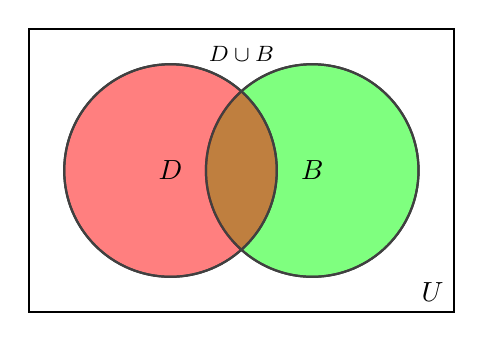
\begin{tikzpicture}[scale=.9]
	\def\circleA{(0,0) circle (1.5)} %A
	\def\circleB{(0:2) circle (1.5)} %B

	\colorlet{circle edgeA}{black!75} 
	\colorlet{circle areaA}{red!100}
	\colorlet{circle edgeB}{black!75} 
	\colorlet{circle areaB}{green!100}

	\tikzset{
		filledA/.style={fill=circle areaA, draw=circle edgeA, thick},
		filledB/.style={fill=circle areaB, draw=circle edgeB, thick},
		outlineA/.style={draw=circle edgeA, thick},
		outlineB/.style={draw=circle edgeB, thick},
	}

	\begin{scope}[fill opacity=0.5]         
			\fill[filledB] \circleB;    
			\fill[filledA] \circleA;
	\end{scope}

	\draw[outlineA] \circleA node {$D$}; 
	\draw[outlineB] \circleB node {$B$}; 
	\node[above=-3pt] at (current bounding box.north) {\footnotesize $D \cup B$}; 
	\draw[thick] (-2,-2) rectangle (4,2) node[anchor=south east] at (current bounding box.south east) {$U$}; 
\end{tikzpicture} }\only<11->{%%%%(AUB)' complement%%%%%
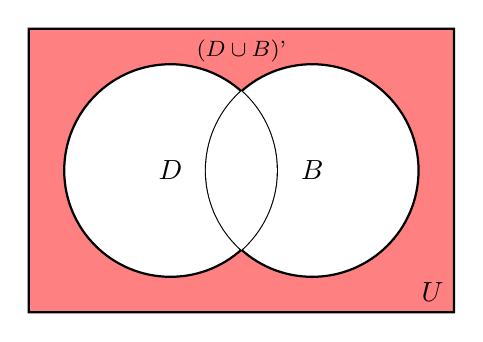
\begin{tikzpicture}[scale=.9]
	\def\circleA{(0,0) circle (1.5)} %A
	\def\circleB{(0:2) circle (1.5)} %B

	\colorlet{circle edgeA}{black!75} 
	\colorlet{circle areaA}{red!100}
	\colorlet{circle edgeB}{black!75} 
	\colorlet{circle areaB}{blue!100}

	\tikzset{
		filledA/.style={fill=circle areaA, draw=circle edgeA, thick},
		filledB/.style={fill=circle areaB, draw=circle edgeB, thick},
		outlineA/.style={draw=circle edgeA, thick},
		outlineB/.style={draw=circle edgeB, thick},
	}

		\draw[thick,fill=red!50,even odd rule] %%even odd rule draws complement of next draw commands%%
			(-2,-2) rectangle (4,2) node[anchor=south east] at (current bounding box.south east) {$U$}
			\circleA node {$D$} \circleB node {$B$};

		\scope 
			\clip (0,0) circle (1.5);%%why can't i use circleA?
			\fill[white] (0:2) circle (1.5); 
		\endscope
		
	\node[below=1pt] at (current bounding box.north) {\footnotesize $(D \cup B$)'}; 

\end{tikzpicture} }

\only<4-5>{
\begin{block}<4-5>{Complement Rule}

\begin{itemize}
\item $n(A)+n(A')=n(U)$

\begin{itemize}
\item $n(A)=n(U)-n(A')$
\item $n(A')=n(U)-n(A)$
\end{itemize}
\end{itemize}
\end{block}
}

\only<6-9>{
\begin{block}<8-9>{Union Rule}

\begin{itemize}
\item $n(A\cup B)=n(A)+n(B)-n(A\cap B)$
\item $n(A\cap B)=n(A\cup B)-n(A)-n(B)$
\end{itemize}
\end{block}
}

\only<10->{
\begin{itemize}
\item How many have neither a DVD or Blue Ray player?

\begin{itemize}
\item <12->[]$n\left((D\cup B)'\right)=n(U)-n(D\cup B)$
\end{itemize}
\end{itemize}
}
\end{columns}
\end{frame}

\begin{frame}{Difference of Sets}

\begin{block}{Difference of Sets}\begin{center}$B-A=\{x\mid x\in B\mbox{ but }x\notin A\}$\end{center}
\end{block}
\begin{center}
%%%blank%%%
\only<2-2>{%%%%A colored; B colored%%%%%
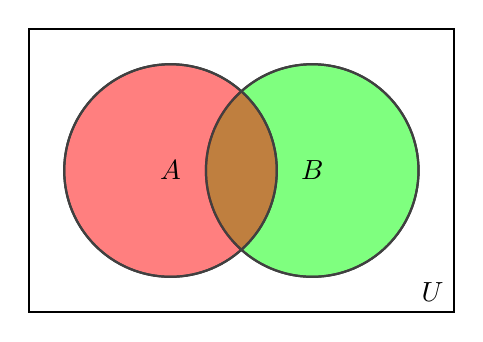
\begin{tikzpicture}[scale=.9]
	\def\circleA{(0,0) circle (1.5)} %A
	\def\circleB{(0:2) circle (1.5)} %B

	\colorlet{circle edgeA}{black!75} 
	\colorlet{circle areaA}{red!100}
	\colorlet{circle edgeB}{black!75} 
	\colorlet{circle areaB}{green!100}

	\tikzset{
		filledA/.style={fill=circle areaA, draw=circle edgeA, thick},
		filledB/.style={fill=circle areaB, draw=circle edgeB, thick},
		outlineA/.style={draw=circle edgeA, thick},
		outlineB/.style={draw=circle edgeB, thick},
	}

	\begin{scope}[fill opacity=0.5]         
			\fill[filledB] \circleB;    
			\fill[filledA] \circleA;
	\end{scope}

	\draw[outlineA] \circleA node {$A$}; 
	\draw[outlineB] \circleB node {$B$}; 
	%\node[anchor=south] at (current bounding box.north) {$A \cup B$}; 
	\draw[thick] (-2,-2) rectangle (4,2) node[anchor=south east] at (current bounding box.south east) {$U$}; 
\end{tikzpicture} }\only<3->{%%%%A-B%%%%%
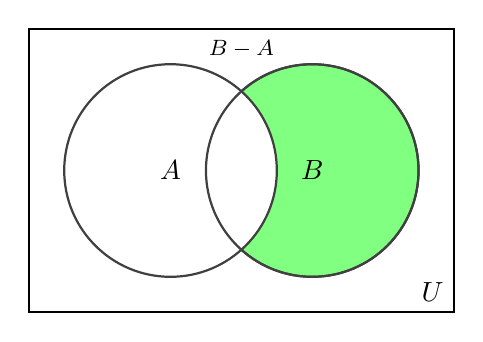
\begin{tikzpicture}[scale=.9]
	\def\circleA{(0,0) circle (1.5)} %A
	\def\circleB{(0:2) circle (1.5)} %B

	\colorlet{circle edgeA}{black!75} 
	\colorlet{circle areaA}{red!50}
	\colorlet{circle edgeB}{black!75} 
	\colorlet{circle areaB}{green!50}

	\tikzset{
		filledA/.style={fill=circle areaA, draw=circle edgeA, thick},
		filledB/.style={fill=circle areaB, draw=circle edgeB, thick},
		outlineA/.style={draw=circle edgeA, thick},
		outlineB/.style={draw=circle edgeB, thick},
	}

	\begin{scope}[shift={(6cm,0cm)}]         
		\begin{scope}[even odd rule]% B-A             
			\clip \circleA (-2,-2) rectangle (4,2);
			\fill[filledB]\circleB;         
		\end{scope}         
		\draw[outlineB] \circleB node {$B$};         
		\draw[outlineA] \circleA node {$A$};
		\draw[thick] (-2,-2) rectangle (4,2) node[anchor=south east] at (current bounding box.south east) {$U$};
	\end{scope}
		
	\node[below=1pt] at (current bounding box.north) {\footnotesize $B-A$}; 

\end{tikzpicture} }
\end{center}
\begin{itemize}
\item <4->$n(B-A)=n(B)-n(A\cap B)$
\item <5->$n(A\cup B)=n(A)+n(B-A)$
\end{itemize}
\end{frame}

\begin{frame}{Counting: two sets}

\ex{1}{}{A store survey of $428$ shoppers finds that: $214$ shoppers made a purchase, $299$ were satisfied with the service they received. Also $52$ of those who made a purchase were not satisfied with the service they received.}
\begin{itemize}
\item [a.] What percentage of shoppers made a purchase and were satisfied
with the service?
\item [b.] What percentage of shoppers made a purchase or were satisfied
with the service?
\item [c.] What percentage of shoppers were satisfied with the service
but did not make a purchase?
\item [d.] What percentage of shoppers were not satisfied and did not make
a purchase?
\end{itemize}
\end{frame}

\begin{frame}{Counting: two sets}

\begin{itemize}
\item []\center{%%%union%%%
\only<1->{%%%%A uncolored; B uncolored%%%%%
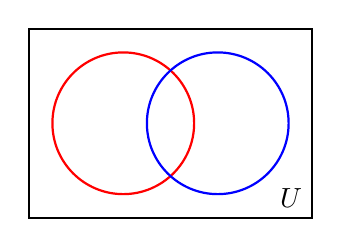
\begin{tikzpicture}[scale=.6]
	\def\circleA{(0,0) circle (1.5)} %A
	\def\circleB{(0:2) circle (1.5)} %B

	\colorlet{circle edgeA}{black!75} 
	\colorlet{circle areaA}{red!100}
	\colorlet{circle edgeB}{black!75} 
	\colorlet{circle areaB}{green!100}

	\tikzset{
		filledA/.style={fill=circle areaA, draw=circle edgeA, thick},
		filledB/.style={fill=circle areaB, draw=circle edgeB, thick},
		outlineA/.style={draw=circle edgeA, thick, red},
		outlineB/.style={draw=circle edgeB, thick, blue},
	}

	\begin{scope}[fill opacity=0.5]         
			%\fill[filledB] \circleB;    
			%\fill[filledA] \circleA;
	\end{scope}

	\draw[outlineA] \circleA node {$$}; 
	\draw[outlineB] \circleB node {$$}; 
	%\node[anchor=south] at (current bounding box.north) {$A \cup B$}; 
	\draw[thick] (-2,-2) rectangle (4,2) node[anchor=south east] at (current bounding box.south east) {$U$}; 
\end{tikzpicture} }}
\item [a.] What percentage of shoppers made a purchase and were satisfied
with the service?
\end{itemize}
\only<2-4>{First define some subsets of $U$. 
\begin{itemize}
\item []<3->$P=\{\mbox{shopper}\mid\mbox{shopper made a purchase}\}$,
$n(P)=214$
\item []<4->$S=\{\mbox{shopper}\mid\mbox{shopper was satisifed with service}\}$,
$n(S)=299$
\end{itemize}
}

\only<5->{$P$ AND $S$$\Rightarrow P\cap S$
\begin{itemize}
\item []<6->The number in $P-S$ is $52$, so
\item []<7->$n(P\cap S)$\only<8->{$=n(P)-52$} \only<9->{$=162$}
\item []<10->,and $\frac{162}{428}\approx.3785=37.85\%$
\end{itemize}
}
\end{frame}

\begin{frame}{Counting: two sets}

\begin{itemize}
\item []\center{%%%union%%%
\only<1->{%%%%A uncolored; B uncolored%%%%%
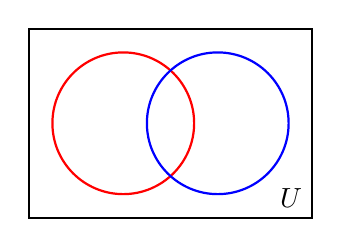
\begin{tikzpicture}[scale=.6]
	\def\circleA{(0,0) circle (1.5)} %A
	\def\circleB{(0:2) circle (1.5)} %B

	\colorlet{circle edgeA}{black!75} 
	\colorlet{circle areaA}{red!100}
	\colorlet{circle edgeB}{black!75} 
	\colorlet{circle areaB}{green!100}

	\tikzset{
		filledA/.style={fill=circle areaA, draw=circle edgeA, thick},
		filledB/.style={fill=circle areaB, draw=circle edgeB, thick},
		outlineA/.style={draw=circle edgeA, thick, red},
		outlineB/.style={draw=circle edgeB, thick, blue},
	}

	\begin{scope}[fill opacity=0.5]         
			%\fill[filledB] \circleB;    
			%\fill[filledA] \circleA;
	\end{scope}

	\draw[outlineA] \circleA node {$$}; 
	\draw[outlineB] \circleB node {$$}; 
	%\node[anchor=south] at (current bounding box.north) {$A \cup B$}; 
	\draw[thick] (-2,-2) rectangle (4,2) node[anchor=south east] at (current bounding box.south east) {$U$}; 
\end{tikzpicture} }}
\item [b.] What percentage of shoppers made a purchase or were satisfied
with the service?
\end{itemize}
\only<2->{$P$ OR $S$$\Rightarrow P\cup S$
\begin{itemize}
\item []<3->$n(P\cup S)=n(P)+n(S)-n(P\cap S)$
\item []<4->$n(P\cup S)$\only<5->{$=214+299-162$} \only<6->{$=351$}
\item []<7->,and $\frac{351}{428}\approx.8201=82.01\%$
\end{itemize}
}
\end{frame}

\begin{frame}{Counting: two sets}

\begin{itemize}
\item []\center{%%%union%%%
\only<1->{%%%%A uncolored; B uncolored%%%%%
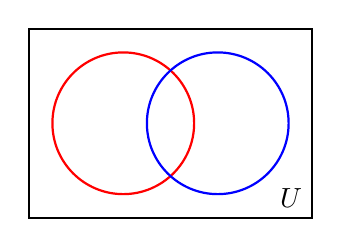
\begin{tikzpicture}[scale=.6]
	\def\circleA{(0,0) circle (1.5)} %A
	\def\circleB{(0:2) circle (1.5)} %B

	\colorlet{circle edgeA}{black!75} 
	\colorlet{circle areaA}{red!100}
	\colorlet{circle edgeB}{black!75} 
	\colorlet{circle areaB}{green!100}

	\tikzset{
		filledA/.style={fill=circle areaA, draw=circle edgeA, thick},
		filledB/.style={fill=circle areaB, draw=circle edgeB, thick},
		outlineA/.style={draw=circle edgeA, thick, red},
		outlineB/.style={draw=circle edgeB, thick, blue},
	}

	\begin{scope}[fill opacity=0.5]         
			%\fill[filledB] \circleB;    
			%\fill[filledA] \circleA;
	\end{scope}

	\draw[outlineA] \circleA node {$$}; 
	\draw[outlineB] \circleB node {$$}; 
	%\node[anchor=south] at (current bounding box.north) {$A \cup B$}; 
	\draw[thick] (-2,-2) rectangle (4,2) node[anchor=south east] at (current bounding box.south east) {$U$}; 
\end{tikzpicture} }}
\end{itemize}
\ex{1}{}{In a 4-H club, $13$ had rabbits, $10$ goats, $4$ had both rabbits and goats, $18$ had neither rabbits nor goats.}
\begin{itemize}
\item [a.] What percentage of members had rabbits or goats?
\item [b.] What percentage of members had only rabbits?
\item [c.] What percentage of members had only goats?
\end{itemize}
\end{frame}

\begin{frame}{Counting: Three Sets}

\begin{figure}
\begin{center}

\def\firstcircle{(90:1.75cm) circle (2.5cm)} 
\def\secondcircle{(210:1.75cm) circle (2.5cm)} 
\def\thirdcircle{(330:1.75cm) circle (2.5cm)}

\begin{tikzpicture}[scale=.9]    
\begin{scope}     
	\fill[red]\firstcircle;       
	\fill[green] \secondcircle;       
	\fill[blue] \thirdcircle;     
\end{scope}     
\begin{scope}
	\clip 
	\secondcircle;       
	\fill[yellow] 
	\firstcircle;     
\end{scope}     
\begin{scope}       
	\clip 
	\secondcircle;       
	\fill[cyan] 
	\thirdcircle;     
\end{scope}     
\begin{scope}       
	\clip 
	\firstcircle;       
	\fill[magenta] 
	\thirdcircle;     
\end{scope}     
\begin{scope}       
	\clip \firstcircle;       
	\clip \secondcircle;       
	\fill[white] \thirdcircle;     
\end{scope}     
\draw 
	\firstcircle node[text=white] {$A$};     
	\draw \secondcircle node [text=white,below left] {$B$};     
	\draw \thirdcircle node [text=white,below right] {$C$};     
\begin{scope}[font=\small]       
	\node(0,0) {$A\cap B\cap C$};       
	\draw(30:1.5cm) node {$A\cap C$};       
	\draw(150:1.5cm) node {$A\cap B$};       
\draw(270:1.5cm) node {$B\cap C$};     
\end{scope}

\draw[thick] (-4.8,-3.55) rectangle (4.75,4.4) node[anchor=south east] at (current bounding box.south east) {$U$}; 

\end{tikzpicture}

\end{center}

\caption{Three Sets}
\end{figure}

\end{frame}

\begin{frame}{Counting: Three Sets}

\vspace{-.5cm}

\ex{1}{}{In an allegry clinic, all patients are allegeric as follows: $70$ to dairy, $100$ to pollen, $80$ to animals, $30$ to all three, $20$ only to pollen, $10$ only to dairy, and $50$ to  dairy and pollen.}

\begin{center}

\def\firstcircle{(90:1.75cm) circle (2.5cm)} 
\def\secondcircle{(210:1.75cm) circle (2.5cm)} 
\def\thirdcircle{(330:1.75cm) circle (2.5cm)}

\begin{tikzpicture}[scale=.75]    
\begin{scope}     
	\fill[red!85]\firstcircle;       
	\fill[green!85] \secondcircle;       
	\fill[blue!85] \thirdcircle;     
\end{scope}     
\begin{scope}
	\clip 
	\secondcircle;       
	\fill[yellow] 
	\firstcircle;     
\end{scope}     
\begin{scope}       
	\clip 
	\secondcircle;       
	\fill[cyan] 
	\thirdcircle;     
\end{scope}     
\begin{scope}       
	\clip 
	\firstcircle;       
	\fill[magenta] 
	\thirdcircle;     
\end{scope}     
\begin{scope}       
	\clip \firstcircle;       
	\clip \secondcircle;       
	\fill[white] \thirdcircle;     
\end{scope}     
	\draw \firstcircle node[text=white] {$D$};    
	\draw \secondcircle node [text=white,below left] {$P$};     
	\draw \thirdcircle node [text=white,below right] {$A$};

\draw[thick] (-4.8,-3.55) rectangle (4.75,4.4) node[anchor=south east] at (current bounding box.south east) {$U$}; 

\end{tikzpicture}

\end{center}
\end{frame}

\begin{frame}{Counting: Three Sets}

\vspace{-.5cm}
\begin{itemize}
\item <2->[a.] What percent of the patients are allergic to dairy?
\item <3->[b.] What percent of the patients are allergic only to dairy?
\item <4->[c.]What percent of the patients are allergic only to dairy and
animals?
\end{itemize}
\begin{center}

\def\firstcircle{(90:1.75cm) circle (2.5cm)} 
\def\secondcircle{(210:1.75cm) circle (2.5cm)} 
\def\thirdcircle{(330:1.75cm) circle (2.5cm)}

\begin{tikzpicture}[scale=.75]    
\begin{scope}     
	\fill[red!85]\firstcircle;       
	\fill[green!85] \secondcircle;       
	\fill[blue!85] \thirdcircle;     
\end{scope}     
\begin{scope}
	\clip 
	\secondcircle;       
	\fill[yellow] 
	\firstcircle;     
\end{scope}     
\begin{scope}       
	\clip 
	\secondcircle;       
	\fill[cyan] 
	\thirdcircle;     
\end{scope}     
\begin{scope}       
	\clip 
	\firstcircle;       
	\fill[magenta] 
	\thirdcircle;     
\end{scope}     
\begin{scope}       
	\clip \firstcircle;       
	\clip \secondcircle;       
	\fill[white] \thirdcircle;     
\end{scope}     
	\draw \firstcircle node[text=white] {$D$};    
	\draw \secondcircle node [text=white,below left] {$P$};     
	\draw \thirdcircle node [text=white,below right] {$A$};

\draw[thick] (-4.8,-3.55) rectangle (4.75,4.4) node[anchor=south east] at (current bounding box.south east) {$U$}; 

\end{tikzpicture}

\end{center}
\end{frame}

\begin{frame}{De Morgan's Laws}

\begin{block}{distribution}

\begin{center}
\begin{itemize}
\item <2-> $a(b+c)=ab+ac$
\item <3->[ex.] $3(x+2)=3x+6$
\end{itemize}
\end{center}

\end{block}
\begin{columns}


\column{5.5cm}
\begin{itemize}
\item <4->Does $\left(A\cup B\right)'=A'\cup B'$?
\item []<5->No, in general.
\item []
\item []
\item <7->Does $\left(A\cap B\right)'=A'\cap B'$?
\item []<8->No, in general.
\end{itemize}

\column{6cm}
\begin{itemize}
\item [ex.]<6->If $A=\{a,b,c\}$, $B=\{b,c\}$, and $U=\{a,b,c,d\}$ then...
\item []
\item []
\item [ex.]<9->If $A=\{a,b,c\}$, $B=\{b,c\}$, and $U=\{a,b,c,d\}$ then...
\end{itemize}
\end{columns}
\end{frame}

\begin{frame}{De Morgan's Laws}

\begin{block}{De Morgan's Laws}

\begin{center}
\begin{itemize}
\item $(A\cup B)'=A'\cap B'$
\item $(A\cap B)'=A'\cup B'$
\end{itemize}
\end{center}

\end{block}
\begin{columns}


\column{5.5cm}

\only<2-2>{%%%%A or B%%%%%
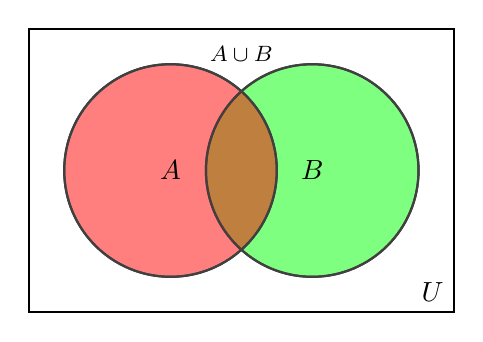
\begin{tikzpicture}[scale=.9]
	\def\circleA{(0,0) circle (1.5)} %A
	\def\circleB{(0:2) circle (1.5)} %B

	\colorlet{circle edgeA}{black!75} 
	\colorlet{circle areaA}{red!100}
	\colorlet{circle edgeB}{black!75} 
	\colorlet{circle areaB}{green!100}

	\tikzset{
		filledA/.style={fill=circle areaA, draw=circle edgeA, thick},
		filledB/.style={fill=circle areaB, draw=circle edgeB, thick},
		outlineA/.style={draw=circle edgeA, thick},
		outlineB/.style={draw=circle edgeB, thick},
	}

	\begin{scope}[fill opacity=0.5]         
			\fill[filledB] \circleB;    
			\fill[filledA] \circleA;
	\end{scope}

	\draw[outlineA] \circleA node {$A$}; 
	\draw[outlineB] \circleB node {$B$}; 
	\node[above=-3pt] at (current bounding box.north) {\footnotesize $A \cup B$}; 
	\draw[thick] (-2,-2) rectangle (4,2) node[anchor=south east] at (current bounding box.south east) {$U$}; 
\end{tikzpicture} }

\only<3-6>{%%%%(AUB)' complement%%%%%
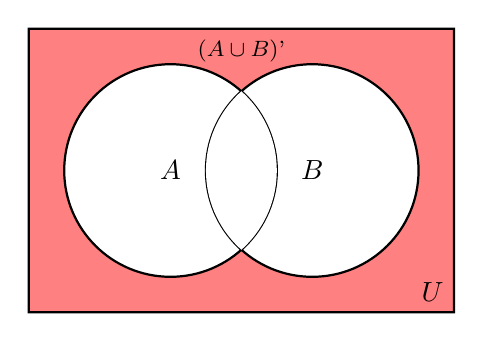
\begin{tikzpicture}[scale=.9]
	\def\circleA{(0,0) circle (1.5)} %A
	\def\circleB{(0:2) circle (1.5)} %B

	\colorlet{circle edgeA}{black!75} 
	\colorlet{circle areaA}{red!100}
	\colorlet{circle edgeB}{black!75} 
	\colorlet{circle areaB}{blue!100}

	\tikzset{
		filledA/.style={fill=circle areaA, draw=circle edgeA, thick},
		filledB/.style={fill=circle areaB, draw=circle edgeB, thick},
		outlineA/.style={draw=circle edgeA, thick},
		outlineB/.style={draw=circle edgeB, thick},
	}

		\draw[thick,fill=red!50,even odd rule] %%even odd rule draws complement of next draw commands%%
			(-2,-2) rectangle (4,2) node[anchor=south east] at (current bounding box.south east) {$U$}
			\circleA node {$A$} \circleB node {$B$};

		\scope 
			\clip (0,0) circle (1.5);%%why can't i use circleA?
			\fill[white] (0:2) circle (1.5); 
		\endscope
		
	\node[below=1pt] at (current bounding box.north) {\footnotesize $(A \cup B$)'}; 

\end{tikzpicture} }

%%next law%
\only<7-7>{%%%%A n B%%%%%
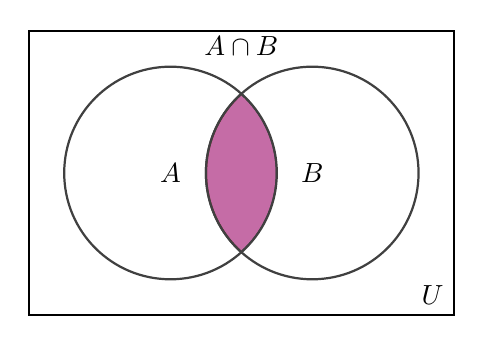
\begin{tikzpicture}[scale=.9]
	\def\circleA{(0,0) circle (1.5)} %A
	\def\circleB{(0:2) circle (1.5)} %B

	\colorlet{circle edgeA}{black!75} 
	\colorlet{circle areaA}{red!100}
	\colorlet{circle edgeB}{black!75} 
	\colorlet{circle areaB}{blue!100}

	\tikzset{
		filledA/.style={fill=circle areaA, draw=circle edgeA, thick},
		filledB/.style={fill=circle areaB, draw=circle edgeB, thick},
		outlineA/.style={draw=circle edgeA, thick},
		outlineB/.style={draw=circle edgeB, thick},
	}
	
	\begin{scope}[fill opacity=0.35]    
		\clip \circleA;     
			\fill[filledB] \circleB;
		\clip \circleB;     
			\fill[filledA] \circleA;
	\end{scope}

	\draw[outlineA] \circleA node {$A$}; 
	\draw[outlineB] \circleB node {$B$}; 
	\node[anchor=south] at (current bounding box.north) {$A \cap B$}; 
	\draw[thick] (-2,-2) rectangle (4,2) node[anchor=south east] at (current bounding box.south east) {$U$}; 
\end{tikzpicture} }

\only<8->{%%%%(A n B)'%%%%%
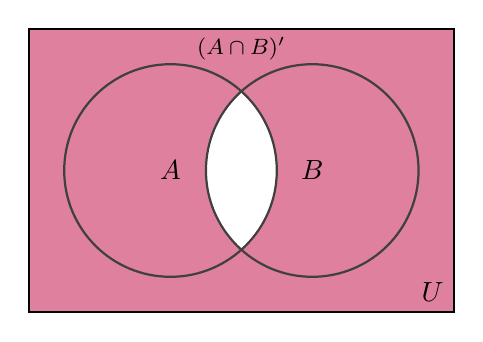
\begin{tikzpicture}[scale=.9]
	\def\circleA{(0,0) circle (1.5)} %A
	\def\circleB{(0:2) circle (1.5)} %B

	\colorlet{circle edgeA}{black!75} 
	\colorlet{circle areaA}{red!100}
	\colorlet{circle edgeB}{black!75} 
	\colorlet{circle areaB}{blue!100}

	\tikzset{
		filledA/.style={fill=circle areaA, draw=circle edgeA, thick},
		filledB/.style={fill=circle areaB, draw=circle edgeB, thick},
		outlineA/.style={draw=circle edgeA, thick},
		outlineB/.style={draw=circle edgeB, thick},
	}    
		
	\draw[thick,fill=purple!50] (-2,-2) rectangle (4,2) node[anchor=south east] at (current bounding box.south east) {$U$};

	\scope 
		\clip \circleA; 		\fill[white] \circleB; 	\endscope

	\draw[outlineA] \circleA node {$A$}; 
	\draw[outlineB] \circleB node {$B$}; 
	\node[anchor=north] at (current bounding box.north) {\footnotesize $(A \cap B)'$};  
\end{tikzpicture} }


\column{.5cm}

\vspace{1.3cm}\only<6-6>{$=$}\only<10->{$=$}

\column{5.5cm}

\only<4-4>{%%%%A complement with B%%%%%
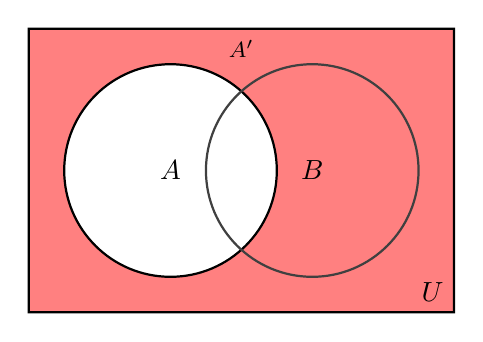
\begin{tikzpicture}[scale=.9]
	\def\circleA{(0,0) circle (1.5)} %A
	\def\circleB{(0:2) circle (1.5)} %B

	\colorlet{circle edgeA}{black!75} 
	\colorlet{circle areaA}{red!100}
	\colorlet{circle edgeB}{black!75} 
	\colorlet{circle areaB}{blue!100}

	\tikzset{
		filledA/.style={fill=circle areaA, draw=circle edgeA, thick},
		filledB/.style={fill=circle areaB, draw=circle edgeB, thick},
		outlineA/.style={draw=circle edgeA, thick},
		outlineB/.style={draw=circle edgeB, thick},
	}

	\draw[thick,fill=red!50,even odd rule] %%even odd rule draws complement of next draw commands%%	 
		(-2,-2) rectangle (4,2) node[anchor=south east] at (current bounding box.south east) {$U$} 
		\circleA node {$A$};
	\draw[outlineB] \circleB node {$B$};
	\node[below=1pt] at (current bounding box.north) {\footnotesize $A'$}; 

\end{tikzpicture} }

\only<5-5>{%%%%A'n B'%%%%%
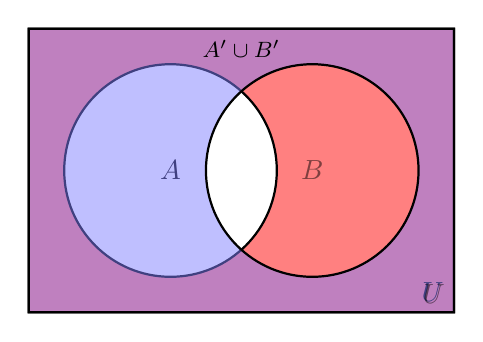
\begin{tikzpicture}[scale=.9]
	\def\circleA{(0,0) circle (1.5)} %A
	\def\circleB{(0:2) circle (1.5)} %B

	\colorlet{circle edgeA}{black!75} 
	\colorlet{circle areaA}{red!100}
	\colorlet{circle edgeB}{black!75} 
	\colorlet{circle areaB}{blue!100}

	\tikzset{
		filledA/.style={fill=circle areaA, draw=circle edgeA, thick},
		filledB/.style={fill=circle areaB, draw=circle edgeB, thick},
		outlineA/.style={draw=circle edgeA, thick},
		outlineB/.style={draw=circle edgeB, thick},
	}

	\draw[thick,fill=red!50,even odd rule] %%even odd rule draws complement of next draw commands%%
		(-2,-2) rectangle (4,2) node[anchor=south east] at (current bounding box.south east) {$U$} 
		\circleA node {$A$};
	
	\tikzset{
		filledB/.style={fill=circle areaB, draw=circle edgeB, thick},
		filledA/.style={fill=circle areaA, draw=circle edgeA, thick},
		outlineB/.style={draw=circle edgeB, thick},
		outlineA/.style={draw=circle edgeA, thick},
	}

\begin{scope}[fill opacity=0.5]  
	\draw[thick,fill=blue!50,even odd rule] %%even odd rule draws complement of next draw commands%%
		(-2,-2) rectangle (4,2) node[anchor=south east] at (current bounding box.south east) {$U$} 
		\circleB node {$B$};
\end{scope}

	\node[below=1pt] at (current bounding box.north) {\footnotesize $A' \cup B'$}; 

\end{tikzpicture} }

\only<6-6>{%%%%A'nB' complement%%%%%
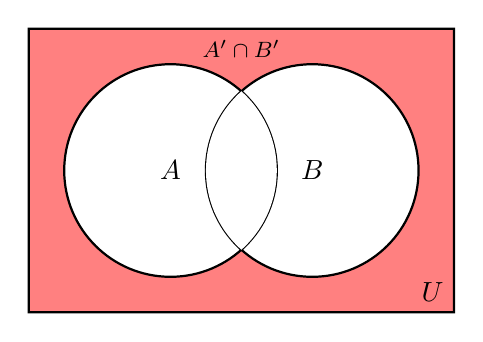
\begin{tikzpicture}[scale=.9]
	\def\circleA{(0,0) circle (1.5)} %A
	\def\circleB{(0:2) circle (1.5)} %B

	\colorlet{circle edgeA}{black!75} 
	\colorlet{circle areaA}{red!100}
	\colorlet{circle edgeB}{black!75} 
	\colorlet{circle areaB}{blue!100}

	\tikzset{
		filledA/.style={fill=circle areaA, draw=circle edgeA, thick},
		filledB/.style={fill=circle areaB, draw=circle edgeB, thick},
		outlineA/.style={draw=circle edgeA, thick},
		outlineB/.style={draw=circle edgeB, thick},
	}

		\draw[thick,fill=red!50,even odd rule] %%even odd rule draws complement of next draw commands%%
			(-2,-2) rectangle (4,2) node[anchor=south east] at (current bounding box.south east) {$U$}
			\circleA node {$A$} \circleB node {$B$};

		\scope 
			\clip (0,0) circle (1.5);%%why can't i use circleA?
			\fill[white] (0:2) circle (1.5); 
		\endscope
		
	\node[below=1pt] at (current bounding box.north) {\footnotesize $A' \cap B'$}; 

\end{tikzpicture} }

%%%next law%%
\only<9-9>{%%%%A complement%%%%%
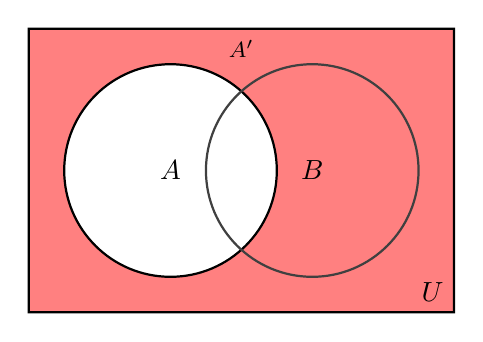
\begin{tikzpicture}[scale=.9]
	\def\circleA{(0,0) circle (1.5)} %A
	\def\circleB{(0:2) circle (1.5)} %B

	\colorlet{circle edgeA}{black!75} 
	\colorlet{circle areaA}{red!100}
	\colorlet{circle edgeB}{black!75} 
	\colorlet{circle areaB}{blue!100}

	\tikzset{
		filledA/.style={fill=circle areaA, draw=circle edgeA, thick},
		filledB/.style={fill=circle areaB, draw=circle edgeB, thick},
		outlineA/.style={draw=circle edgeA, thick},
		outlineB/.style={draw=circle edgeB, thick},
	}

	\draw[thick,fill=red!50,even odd rule] %%even odd rule draws complement of next draw commands%%	 
		(-2,-2) rectangle (4,2) node[anchor=south east] at (current bounding box.south east) {$U$} 
		\circleA node {$A$};
	\draw[outlineB] \circleB node {$B$};
	\node[below=1pt] at (current bounding box.north) {\footnotesize $A'$}; 

\end{tikzpicture} }

\only<10-10>{%%%%A'U B'%%%%%
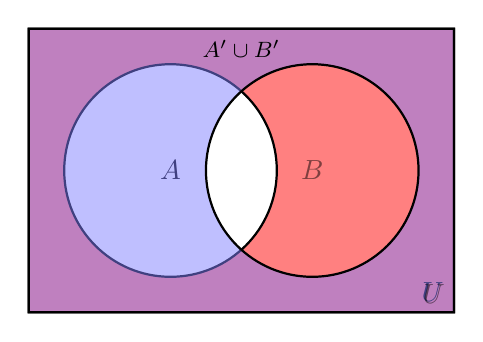
\begin{tikzpicture}[scale=.9]
	\def\circleA{(0,0) circle (1.5)} %A
	\def\circleB{(0:2) circle (1.5)} %B

	\colorlet{circle edgeA}{black!75} 
	\colorlet{circle areaA}{red!100}
	\colorlet{circle edgeB}{black!75} 
	\colorlet{circle areaB}{blue!100}

	\tikzset{
		filledA/.style={fill=circle areaA, draw=circle edgeA, thick},
		filledB/.style={fill=circle areaB, draw=circle edgeB, thick},
		outlineA/.style={draw=circle edgeA, thick},
		outlineB/.style={draw=circle edgeB, thick},
	}

	\draw[thick,fill=red!50,even odd rule] %%even odd rule draws complement of next draw commands%%
		(-2,-2) rectangle (4,2) node[anchor=south east] at (current bounding box.south east) {$U$} 
		\circleA node {$A$};
	
	\tikzset{
		filledB/.style={fill=circle areaB, draw=circle edgeB, thick},
		filledA/.style={fill=circle areaA, draw=circle edgeA, thick},
		outlineB/.style={draw=circle edgeB, thick},
		outlineA/.style={draw=circle edgeA, thick},
	}

\begin{scope}[fill opacity=0.5]  
	\draw[thick,fill=blue!50,even odd rule] %%even odd rule draws complement of next draw commands%%
		(-2,-2) rectangle (4,2) node[anchor=south east] at (current bounding box.south east) {$U$} 
		\circleB node {$B$};
\end{scope}

	\node[below=1pt] at (current bounding box.north) {\footnotesize $A' \cup B'$}; 

\end{tikzpicture} }
\end{columns}
\end{frame}

\begin{frame}{Problems}

\begin{columns}


\column{6cm}

%%%union%%%
\only<1->{%%%%A uncolored; B uncolored%%%%%
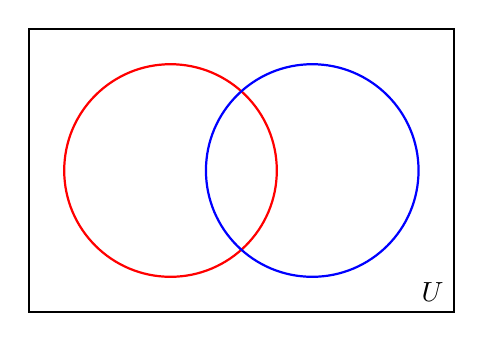
\begin{tikzpicture}[scale=.9]
	\def\circleA{(0,0) circle (1.5)} %A
	\def\circleB{(0:2) circle (1.5)} %B

	\colorlet{circle edgeA}{black!75} 
	\colorlet{circle areaA}{red!100}
	\colorlet{circle edgeB}{black!75} 
	\colorlet{circle areaB}{green!100}

	\tikzset{
		filledA/.style={fill=circle areaA, draw=circle edgeA, thick},
		filledB/.style={fill=circle areaB, draw=circle edgeB, thick},
		outlineA/.style={draw=circle edgeA, thick, red},
		outlineB/.style={draw=circle edgeB, thick, blue},
	}

	\begin{scope}[fill opacity=0.5]         
			%\fill[filledB] \circleB;    
			%\fill[filledA] \circleA;
	\end{scope}

	\draw[outlineA] \circleA node {$$}; 
	\draw[outlineB] \circleB node {$$}; 
	%\node[anchor=south] at (current bounding box.north) {$A \cup B$}; 
	\draw[thick] (-2,-2) rectangle (4,2) node[anchor=south east] at (current bounding box.south east) {$U$}; 
\end{tikzpicture} }
\end{columns}
\prob{1}{1}{Let $U=\{x\mid x\mbox{ is an integer and }0\leq x\leq10\}$, $A=\{0,2,4,6,8,10\}, and $B=\{0,1,2,3,4,5\}.}{Use De Morgan's law to find $(A'\cup B)'$}\prob{2}{2}{Let $U=\{x\mid x\mbox{ is an integer and }0\leq x\leq10\}$, $A=\{0,2,4,6,8,10\}, and $B=\{0,1,2,3,4,5\}.}{Use De Morgan's law to find $(A'\cap B)'$}\prob{3}{3}{Let $U=\{x\mid x\mbox{ is an integer and }0\leq x\leq10\}$, $A=\{0,2,4,6,8,10\}, and $B=\{0,1,2,3,4,5\}.}{Use De Morgan's law to find $(A'\cap B')'$}\prob{4}{4}{Let $U=\{x\mid x\mbox{ is an integer and }0\leq x\leq10\}$, $A=\{0,2,4,6,8,10\}, and $B=\{0,1,2,3,4,5\}.}{Use De Morgan's law to find $(A \cup B')'$}
\end{frame}

\end{document}
